%!TEX root = ../thesis.tex
%*******************************************************************************
%****************************** Fourth Chapter *********************************
%*******************************************************************************
\graphicspath{{Chapter4/Figs/Vector/}{Chapter4/Figs/}}

%%%%%%%%%%%%%%%%%%%%%%%%%%%%%%%%%%%%%%%%%%%%%%%%%%%%%%%%%%%%%%%%%%%%%%%%%%%%%%%%
% Trip Price Calculation System
%%%%%%%%%%%%%%%%%%%%%%%%%%%%%%%%%%%%%%%%%%%%%%%%%%%%%%%%%%%%%%%%%%%%%%%%%%%%%%%%
% - Which logic and data is required in the backend to reliably calculate a
%   trip price?
% #region
\chapter{Trip Price Calculation System}
\section{Introduction}
The term 'rule-based' in the title caters to the proposition that trip price calculations hinge on information defined as something called a rule. This chapter contains resolutions that are less based on empirical evidence and more on the input of the product owner and a balancing of arguments that support important quality attributes. The questions in regard to the implementation of the backend are answered, resulting in a system that deterministically calculates trip prices using rules that are restricted by user defined criteria.
% #endregion

%%%%%%%%%%%%%%%%%%%%%%%%%%%%%%%%%%%%%%%%%%%%%%%%%%%%%%%%%%%%%%%%%%%%%%%%%%%%%%%%
% The System Structure
%%%%%%%%%%%%%%%%%%%%%%%%%%%%%%%%%%%%%%%%%%%%%%%%%%%%%%%%%%%%%%%%%%%%%%%%%%%%%%%%
% #region
\section{The System Structure}
In the previous chapter, the second proof of concept was mentioned that separates the calculation logic from the Loopback framework, as shown in Figure \ref{fig:Class Diagram}. The isolation of the calculation and direction classes result in a more robust system. The Price object is composed of a Directions and a Calculator Class, both of which expose only one method, directions and calculate respectively. The behavior of the gathering of directions information and calculation of prices is encapsulated in different subclasses using the strategy pattern as described in \cite{gof}. Allowing behavior to change on demand. The entities stored in the database are conceptualized in Figure \ref{fig:Data Model}, and will be referenced throughout this chapter. Chapter three concludes that MongoDB is the proper database for this system. MongoDB allows relations to be embedded in the parent's document, which is useful for child entities, like timeframes, that are never shared.

\begin{figure}[H]
	\centering
	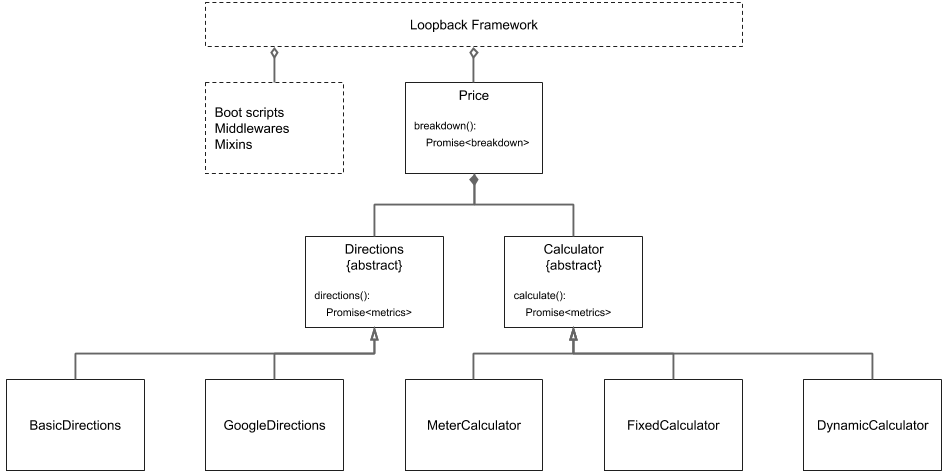
\includegraphics[width=1\textwidth]{ClassDiagram}
	\caption[Class Diagram]{High level class diagram.}
	\label{fig:Class Diagram}
\end{figure}

\begin{figure}[H]
	\centering
	
\includegraphics[width=1\textwidth]{DataModel}
	\caption[Data Model]{Conceptual data model showing database entity relations.}
	\label{fig:Data Model}
\end{figure}
% #endregion

%%%%%%%%%%%%%%%%%%%%%%%%%%%%%%%%%%%%%%%%%%%%%%%%%%%%%%%%%%%%%%%%%%%%%%%%%%%%%%%%
% Matching Criteria
%%%%%%%%%%%%%%%%%%%%%%%%%%%%%%%%%%%%%%%%%%%%%%%%%%%%%%%%%%%%%%%%%%%%%%%%%%%%%%%%
% #region
\section{Matching Criteria}
A rule is the rudimentary element of the trip pricing system that allows users to interpret and define the way with which prices are assigned to trips, restricted by the dimensions of space and time. In the legacy system, discounts were a fundamental part of the price definitions. Meaning that whenever a price was found, the discount was directly associated with the price. This design led to some issues, mainly revolving around having to duplicate prices in order to have the same prices without discounts. It is mutually beneficial for users and developers who are destined to maintain this system, to create a system that offers a lot of freedom in applying criteria to prices. In perspective, a user may want to apply the following restrictions:

\begin{enumerate}
	\item Define certain prices for one app, but not for the other
	\item Define lower dynamic prices in Rotterdam
	\item Define a certain fixed price during New Year's Eve
	\item Assign a discount for trips that depart from Schiphol
	\item Define a higher price for trips that end in larger cities
	\item Make the limousine available only in North Holland
	\item Allow for free trips between two companies during the weekend
\end{enumerate}

There are also some restrictions that are applied by default as pre- or  postconditions. For example, the passenger count should not exceed that of the products' passenger capacity. An on demand option in the booking app allows passengers to book a ride without providing a destination. In these cases, a rule must still be matched with the departure location, and the user may want to disable some products for the on-demand functionality. This is an example where the products are shown without prices, or filtered out if the user wishes it. Compared to the legacy system, this design of allowing criteria to be applied to rules and discounts independently, resulting in a more modular system with more freedom. The user is allowed to define discounts and rules separately, and when a new concept is added that makes use of locations or timeframes, the user is able to reason about it in the same fashion. For the maintainers of this system, it is beneficial to have less duplication, more separation of concern, and less overhead.

\subsection{Locations}
Chapter two concludes that MongoDB's geometry datatypes are sufficient location encodings. The location matching examples can directly be implemented as a basis for the location matching criterion. The listed restrictions that a user may apply, depend on two locations being matched or ignored simultaneously. On top of that, one best match must be selected from the matching results, which must be done by determining what the solution for location overlap should be.

\subsubsection{The Conventional Approach}
The legacy postal code and address based system maintains a type based matching order: fixed, tier, and dynamic rule types. A location conflict would not occur if the user was able to make distinct pricing records. If it were to occur, the system would simply pick the first match. But with the introduction of overlap, this will no longer be feasible. North Holland contains Amsterdam, which contains Amsterdam-Centrum, which contains the Dam Square, which may contain a pickup location defined by the user. There exists some difference in magnitude of locations in the new system, whereas the old system had locations of the same magnitude.

\subsubsection{The New Approach}
Multipolygons allow for multiple locations to be defined as one, opening up the possibility of defining all branches of a company in a single location, which could then be selected as departure and destination location. This would solve example seven from the examples list, using just one rule and one location. Because locations could be associated with all rule types, all location based examples are easy to define. Although care must be taken to distinguish between not having a location defined, and not providing a location when booking a ride. If no departure location is assigned to a rule, the rule should match with any location. And if the passenger orders an on-demand ride, where the destination is not provided, the destination should be ignored during the matching process.

\begin{center}
\noindent\begin{minipage}{.85\textwidth}
\begin{lstlisting}[caption={Matching departure.}, label={lst:matching-departure}]
const query = [];

if (departure) {
	query.push({
		$match: {
			$or: [{
				"departure.area": {
					$geoIntersects: {
						$geometry: {
							type: "Point",
							coordinates: [
								departure.gps.lat,
								departure.gps.lng
							]
						}
					}
				}
			},
			{
				"departure": { $exists: false }
			}]
		}
	})
}

db.collection('Location')
	.aggregate(query)
\end{lstlisting}
\end{minipage}
\end{center}

In Listing \ref{lst:matching-departure}, the query is built conditionally. If a location is not provided by the booking app, it will not be evaluated. Only the provided locations are matched if they intersect with a defined destination, or if the destination does not exists in the database. This covers the cases for checking only one of the two locations. In chapter two, solutions have been proposed to the overlapping locations problem. From all the interesting approaches, the most straight forward solution is simply assigning a priority number to the rule. This solution has the advantage of interpretability and flexibility. The behavior of the matching system can easily be tinkered with by the user. The user can reason about the fact whether one rule has a precedence over the other by comparing the priorities.

\subsection{Timeframes}
The requirements state that the user must be able to define a start and end time, the days on which the times are active, and the start and end date of the timeframe. This either means that the timeframe one window of time, or that each given day has a single window of time. But if a discount should be active during night of New Years Eve, between 23h and 5h, this description would not be sufficient to cover this use case under any interpretation.

\subsubsection{The Conventional Approach}
The legacy system takes a straight forward approach of storing time in a relational database. The begin and end of a window are stored in a record that is related to a parent timeframe entity. The timeframe has many windows that could contain a timestamp. It either finds one or many time windows that contain the timeframe. This approach covers all possibilities imaginable. The downside of this approach is the complexity to interpret or mutate the value of the timeframe.

\subsubsection{The New Approach}
For this reason, a proposal was made to implement timef	rames in a way that let users choose to describe each hour of the week, being stored as a bit map. The windows could be decreased to half an hour, resulting in twice as many bits. Three implementations have been tested, where the bit string format offered the best outcome, as seen in \ref{appendix:slides_4}. A timeframe is stored having two ISODates (international standard: ISO 8601), and a bit string representing the schedule for which the insert statement is shown in Listing \ref{lst:new-timeframe}.

\begin{center}
\noindent\begin{minipage}{.85\textwidth}
\begin{lstlisting}[caption={Improved timeframe.}, label={lst:new-timeframe}]
db.Timeframe.insert({
	startDate: new Date(2018, 4, 7),
	endDate: new Date(2019, 4, 7),
	weekSchedule:
		"001101000110011011000011
		011010110011000010111100
		101010101110100011111000
		111110011111011100100001
		101000000010111011100100
		110010000001000010101101
		010111101000000101001110"
})
\end{lstlisting}
\end{minipage}
\end{center}

A string is a very flexible datatype. Using a regex in a query makes checking multiple bits in the string relatively easy, and enables different values next to 0 and 1. 3. A bit array would only allow for 0 and 1 to be used. A bit string also makes querying the data really stable, as the query will simply not match if the content of the data is not of expected length or value. Performance is not an issue if the regex column is indexed, and when prefix expressions $(/\string^/)$ are used, as per documentation in \cite{MongoDB-Regex}. As noted before, the system is easy to scale if existing data can be migrated to deal with a new amount of bits, or new character usage over bits.

\begin{center}
\noindent\begin{minipage}{.85\textwidth}
\begin{lstlisting}[caption={Opening timeframe.}, label={lst:open-timeframe}]
/**
 * Date object days start at sunday, in order let monday be
 * index 0, decrease the index by one, but limit numbers
 * in the range of [0, 7).
 */
const startMonday = (d: number) => (d - 1) % 7;

/**
 * Creates a regex that spreads bits across hours of each
 * day of the week.
 */
export const regexFromDate = (date: Date) => {

	const skip =
		// Day of the week multiplied by hours a day
		startMonday(date.getDay()) * 24
		// Hour of the day
		+ date.getUTCHours();

	return { skip, timeRegex: new RegExp(`^.{${skip}}1`) };
};
\end{lstlisting}
\end{minipage}
\end{center}

The regexFromDate could be used to create a regex that could be used in a query to check whether a single hour within a week is set. Skip is an integer representing the number of bits that should be skipped to get to the moment represented by the date. So in order to get 11 AM - 12 AM in the presented schedule, 3 * 24 skips + 11 skip = 83 skips are to be made to find the digit 1 on thursday. Because the getDay method on JavaScript date objects return an integer resembling the day, starting at sunday, the startMonday function is used to pretend that it starts on monday.
% #endregion

%%%%%%%%%%%%%%%%%%%%%%%%%%%%%%%%%%%%%%%%%%%%%%%%%%%%%%%%%%%%%%%%%%%%%%%%%%%%%%%%
% The Trip Price Calculation
%%%%%%%%%%%%%%%%%%%%%%%%%%%%%%%%%%%%%%%%%%%%%%%%%%%%%%%%%%%%%%%%%%%%%%%%%%%%%%%%
% #region
\section{The Trip Price Calculation}
The process from start to end is has many edge- and corner cases. Three major stages of the process: handling the incoming request, finding the matching price rule, and calculating the prices, are explained concisely in the following subsections to provide a general overview. Important details of calculation types will be expanded upon in later sections of this chapter.

\subsection{Incoming Request}
The flowchart in Figure \ref{fig:Incoming Request} shows the point where the request is received, up until the point where enough information is known to fetch rules and discounts from the database. When the request is received (1), the user is authenticated. The JSON Web Token contains the user identity, the companyId and daAppInstallId (2). The request body contains information about the ride: vehicle types, passenger count, requested date, departure, and destination.

\begin{figure}[H]
	\centering
	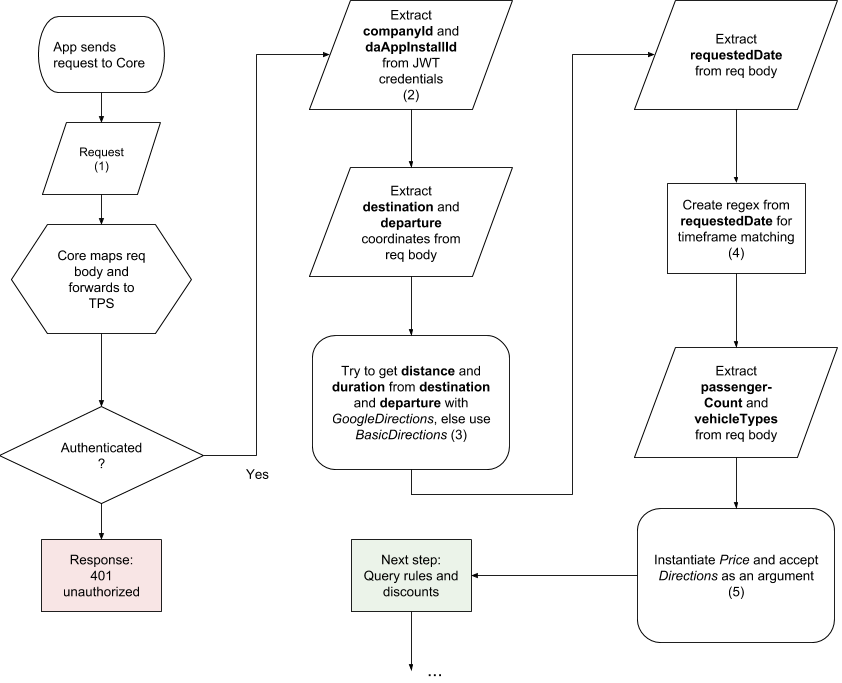
\includegraphics[width=.8\textwidth]{IncomingRequest}
	\caption[Incoming Request]{The condensed flow of a trip price calculation - incoming request.}
	\label{fig:Incoming Request}
\end{figure}

The Directions class will provide an interface to retrieve trip related data. The departure and destination are fed to the Directions class, which will proceed and work out the distance and duration of the trip (3). If the GoogleDirections class is unable to determine the trip details, the BasicDirections class returns a base case result. The trip price calculation flow changes drastically when no destination or departure locations are provided in the request body. Having alternative behaviors helps dealing with providing the most accurate information possible. The strategy pattern also improves the systems resistance to change. If a different service is needed to determine the trip details in the future, it can easily take the place of one of the current services. If the trip details have not been obtained, but at least one of the two, departure or destination locations, have been provided, a database query could still work out the best matching price rule based on partial information. The requestedDate is to be converted to a regex pattern (4) for reasons explained in the timeframes section of this chapter.

\subsection{Data Aggregation}
When the user is authenticated, the system immediately requests the distance and duration of a ride by providing the departure and destination locations to the directions service. This service awaits the trip details response while it is fed to a Price class instantiation (5). The Price class will wait until matched pricing rules are provided, upon which it will perform the price calculation. Before this is the case, the aggregate queries are performed (6), trying to find a matching rule and discount for a particular company/app combination. Two separate queries start by finding the application and company combination for which a price is calculated. If a reference to a debtor is provided, rules and discounts linked to it are used instead. The rules and discounts contain criteria in the form of timeframes and locations. A discount has basic properties while the rule has complex pricing information for products. Figure \ref{fig:Data Aggregation} shows the most important stages of the rule aggregation pipeline. The discount aggregate is a more simple version and has some of the same stages, its flowchart is therefore excluded.

\begin{figure}[H]
	\centering
	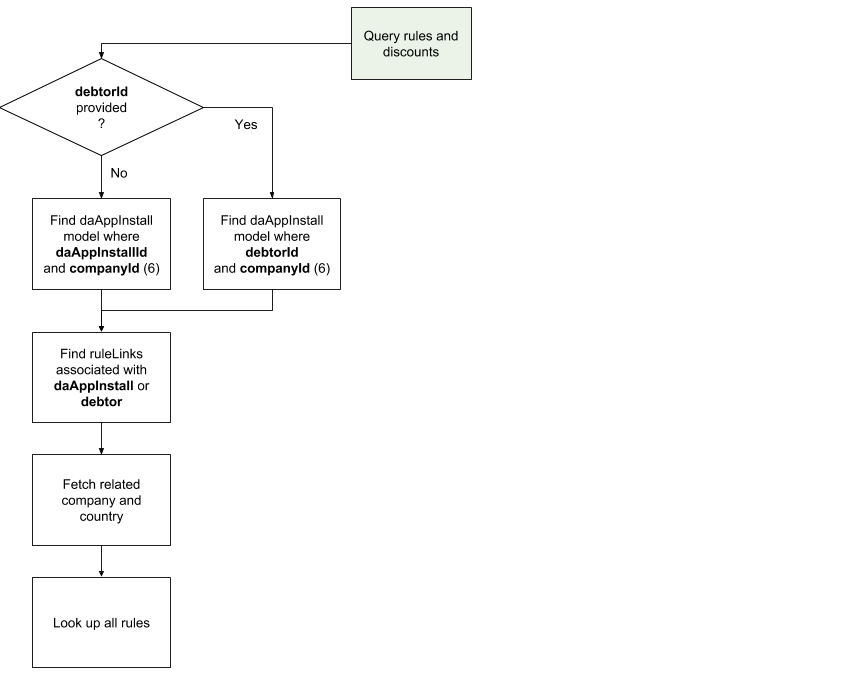
\includegraphics[width=.8\textwidth]{DataAggregation}
	\caption[Data Aggregation]{The condensed flow of a trip price calculation - data aggregation.}
	\label{fig:Data Aggregation}
\end{figure}

\subsection{Calculation}
When both queries have finished, potential discounts are added to each pricing rule, which are then fed to the Price class asynchronously. A single rule has price information for each available product of that rule. If a company offers three products, it is possible to only offer two products in a given timeframe or area by associating them with a rule. For each product that is related to the price rule fetched from the database, a price breakdown is calculated. If the array of matched rules is empty, a map over the array will result in an empty array of price breakdowns. Pricing information is validated before the calculation is started using the method shown in Listing \ref{lst:check-pricing-props}. The system should throw an error, as a price calculation can not proceed without the required information.

\begin{center}
\noindent\begin{minipage}{.85\textwidth}
\begin{lstlisting}[caption={Find missing properties.}, label={lst:check-pricing-props}]
/**
 * Check if pricing contains valid properties and is not undefined.
 */
public static validPricingOrError(pricing: pricing | undefined): void {
	if (pricing === undefined) {
		throw new HttpError('Pricing data is undefined.');
	}
	const missing = [
		'prices',
		'rules',
		'country',
		'company',
		'type',
		'maxPassengers',
	].filter(prop => !(prop in pricing));
	if (missing.length) {
		throw new HttpError('Pricing data is missing properties:\n\t' + missing);
	}
}
\end{lstlisting}
\end{minipage}
\end{center}

A price breakdown follows a series of logical steps, in which functions are created that have a certain default behavior. The strategy pattern is once again applied to use the appropriate calculator for the type of calculation that is required. The different types of calculations are discussed in the next chapter.

\begin{figure}[H]
	\centering
	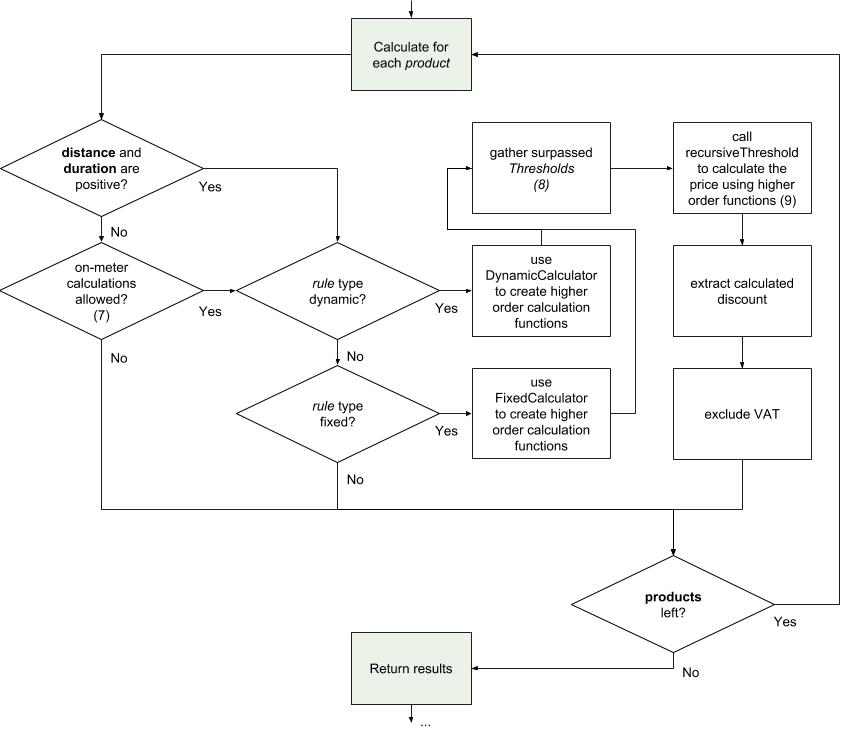
\includegraphics[width=.8\textwidth]{Calculation}
	\caption[Calculation]{The condensed flow of a trip price calculation - calculation.}
	\label{fig:Calculation}
\end{figure}

In step (7) the system faces the issue of not being able to calculate a price, because the distance and duration are not known. In this case, the user is able to choose whether on-meter calculations are allowed to be made, meaning that a meter is used to capture these metrics at a different period of time. If the user agrees, the products are returned with a truthy isAllowedOnMeter flag. The system will still follow the calculation procedure, but will use the MeterCalculator instead of the other two. Step (8) and (9) will be expanded upon in the Threshold Calculations chapter.
% #endregion

%%%%%%%%%%%%%%%%%%%%%%%%%%%%%%%%%%%%%%%%%%%%%%%%%%%%%%%%%%%%%%%%%%%%%%%%%%%%%%%%
% Price Calculation Types
%%%%%%%%%%%%%%%%%%%%%%%%%%%%%%%%%%%%%%%%%%%%%%%%%%%%%%%%%%%%%%%%%%%%%%%%%%%%%%%%
% - What was proposed as a solution to store a week schedule in a database?
% #region
\section{Price Calculation Types}
The calculate method of each calculator subclass receives the pricing information of a product and directions information of a ride. This setup proves to encapsulate all possible calculations that depend on any metric type (distance, duration, ...) and any more complex operation. The calculator method will perform the calculation in a fixed number of steps:

\begin{enumerate}
	\item Define the metrics (and units) for the calculation
	\item Define a lambda function expressed a blueprint to generate a collection of calculator functions
	\item Generate calculator functions that can be used by a deterministic function
	\item Call the deterministic function
	\item Return the total price
\end{enumerate}

\begin{center}
\noindent\begin{minipage}{.85\textwidth}
\begin{lstlisting}[caption={Calculator generator.}, label={lst:calculator-generator}]
/**
 * Generate functions based on prices and units, incorporating
 * default prices that are passed next to different metrics
 * and stored in a indexed object which names are types.
 */
public static generateCalculators(
	prices: indexed,
	metrics: metrics & indexed,
	func: Function,
): object {
	const calculators: indexed = {};
	for (const type in metrics) {
		calculators[type] = (
			price: number = prices[type],
			unit: number = metrics[type],
		) => func(price, unit);
	}
	return calculators;
}
\end{lstlisting}
\end{minipage}
\end{center}

The generateCalculators method generates a function for each metric with default parameters.

\subsection{Dynamic}
A dynamic calculation is performed on the metrics: distance and duration, having units: kilometer and minute. A straight forward lambda expresses that the units are multiplied by the price.

\begin{center}
\noindent\begin{minipage}{.85\textwidth}
\begin{lstlisting}[caption={Dynamic calculation.}, label={lst:dynamic-calculation}]
/**
 * Main calculation for a dynamic pricing rule.
 */
public calculate(
	pricing: pricing,
	metrics: metrics & indexed,
): number {

	const thresholds: threshold[] = pricing.prices.dynamicThresholds;
	const startAmount = pricing.prices.dynamicStartPrice;
	const minAmount = pricing.prices.dynamicMinimumPrice;
	const cascaded = pricing.prices.cascadingThresholdCalculation;

	const prices: indexed = {
		distance: pricing.prices.dynamicDistancePrice,
		duration: pricing.prices.dynamicMinutePrice,
	};

	// Generating calculators
	const func = (price: number, unit: number) => price * unit;
	const calculators = Calculator.generateCalculators(prices, metrics, func);

	// Walk through the thresholds to calculate total price using calculators
	const total = Price.total(
		metrics,
		thresholds,
		calculators,
		cascaded,
	);

	return Math.max(
		total + startAmount,
		minAmount,
	);
}
\end{lstlisting}
\end{minipage}
\end{center}

From this expression, calculators are generated. When a calculator is called without arguments, the default parameter values are used. When the calculator function is called with just the distance, the second default parameter will be the price for that distance. This property is needed for the threshold calculations that are discussed in the next section. The thresholds array contains pricing information for each successive threshold that has been surpassed.

\subsection{Fixed}
Opposed to a dynamic price, the fixed price can not be expressed as a quadratic formula. However, thresholds may increase the price in steps.

\begin{center}
\noindent\begin{minipage}{.85\textwidth}
\begin{lstlisting}[caption={Fixed calculation.}, label={lst:fixed-calculation}]
/**
 * Calculate fixed price.
 */
public calculate(
	pricing: pricing,
	metrics: metrics & indexed,
): number {

	const thresholds: threshold[] = pricing.prices.fixedThresholds;
	const cascaded = false;

	// Price for distance metric only
	const prices: indexed = {
		distance: pricing.prices.fixedPrice,
		duration: 0,
	};

	// Explain how the price should be calculated
	const func = (price: number, unit?: number) => price;

	// Calculator for each metric using prices as default params
	const calculators = Calculator.generateCalculators(prices, metrics, func);

	// Walk through the thresholds to calculate total price using calculators
	const total = Price.total(
		metrics,
		thresholds,
		calculators,
		cascaded,
	);

	// Return biggest of the two
	return Math.max(total, 0);
}
\end{lstlisting}
\end{minipage}
\end{center}

\subsection{Meter}
The meter calculator should return zero under every circumstance.

\begin{center}
\noindent\begin{minipage}{.85\textwidth}
\begin{lstlisting}[caption={Meter calculation.}, label={lst:meter-calculation}]
/**
 * Main calculation for a on meter calculation.
 */
public calculate(
	pricing: pricing,
	metrics: metrics & indexed,
): number {
	return 0;
}
\end{lstlisting}
\end{minipage}
\end{center}

The on-meter calculation simply returns a breakdown for which all values are zero. This is done by convention at taxiID, so that the mobile apps can still display the products that are available, and determine the price at a later stage.
% #endregion

%%%%%%%%%%%%%%%%%%%%%%%%%%%%%%%%%%%%%%%%%%%%%%%%%%%%%%%%%%%%%%%%%%%%%%%%%%%%%%%%
% Threshold Calculations
%%%%%%%%%%%%%%%%%%%%%%%%%%%%%%%%%%%%%%%%%%%%%%%%%%%%%%%%%%%%%%%%%%%%%%%%%%%%%%%%
% #region
\section{Threshold Calculations}
On top of each calculation type, prices can be defined after certain thresholds are surpassed. For example: if a taxi travels 25km, a threshold could be defined at 20km, after which the price will be 10 cents cheaper. In this case, the passenger pays a normal price for the 20 kilometers, and a cheaper price for the last 5 kilometers. This procedure is executed for each metric, but only if the cascading option is specified.  Only the name of the metric used to measure thresholds and the actual calculation functions may change. For this reason, it is possible to define a function that recursively walks through all surpassed thresholds, then calculates a price using different calculations after each threshold was surpassed, as shown in Listing \ref{lst:threshold-recursion}

\begin{center}
\noindent\begin{minipage}{.85\textwidth}
\begin{lstlisting}[caption={Recursive threshold calculation.}, label={lst:threshold-recursion}]
	/**
	* Recursive function that calculates a price for each threshold
	* in a way specified by a calculation function that is passed
	* until the thresholds are empty.
	*/
 public static recursiveThreshold(
	 thresholds: threshold[],
	 calculation: Function,
	 metric: number,
	 cascaded: boolean = true,
 ): number {

	 if (thresholds === undefined || thresholds.length < 1) {
		 log('\tno more thresholds at ' + metric + ', using default price');
		 return calculation(undefined, metric);
	 }

	 log('\tthreshold met at ' + metric);

	 if (!cascaded) {
		 return calculation(thresholds[0].value, metric);
	 }

	 const nextMetric = thresholds[0].threshold;
	 const newMetric = metric - nextMetric;
	 const price = calculation(thresholds[0].value, newMetric);

	 return price + Price.recursiveThreshold(
		 thresholds.slice(1),
		 calculation,
		 nextMetric,
	 );
 }
\end{lstlisting}
\end{minipage}
\end{center}

The Typescript type definitions reveal that calculation is of type Function, and thresholds is of type threshold[]. The base case returns the calculation with an undefined first argument. This forces the calculation method to use its default value, which is actually the normal kilometer or minute price. The base case will have the value of the first threshold that is met, assuring that the passenger pays the normal price up until that point. If the base case is not satisfied, the function checks whether the cascading boolean is true. This boolean determines whether each threshold should be evaluated, or only the last one. In case of the fixed price calculation, only the last threshold fixed price will be computed. But for the dynamic prices, each step has to be added to the total amount. Finally, the calculation is made using the next threshold,  and the recursive call is summed up with the calculated price.
% #endregion

%%%%%%%%%%%%%%%%%%%%%%%%%%%%%%%%%%%%%%%%%%%%%%%%%%%%%%%%%%%%%%%%%%%%%%%%%%%%%%%%
% Determinism
%%%%%%%%%%%%%%%%%%%%%%%%%%%%%%%%%%%%%%%%%%%%%%%%%%%%%%%%%%%%%%%%%%%%%%%%%%%%%%%%
%
\section{Determinism}
A deterministic algorithm always produces the same output given a certain input. This concept is paramount when calculating prices. This does not imply that a criterion is not allowed to change. It does mean that given a certain input and a certain set of criteria, the output should be the same every single time. External state or time are crucial factors that determine whether a function can be deterministic. The concept of determinism is further explained in a later chapter. In the object-oriented programming (OOP) paradigm, state is managed through encapsulation. Object instances manage their internal state, and expose public methods to allow certain changes to be made on those instances. The functional programming (FP) paradigm treats computations as evaluations of mathematical functions. This aspect fits perfectly with the goal of reaching determinism. Using FP in conjunction with OOP, a higher order structure may be implemented using classes and encapsulation for more flexibility, while minimizing or eliminating state mutations through pure functions. Parts of the system may execute operations asynchronously, emphasizing the importance of managing state flawlessly. There are factors that can not be controlled also, such as computations of external services at different times. For example, if a passenger books a ride, and Google's algorithm gives a different estimated distance and duration, the price may go up or down. These factors are side effects that are out of the scope of containment. Side effects that can be contained should be eliminated as much as possible. Professor Frisby demonstrates side effects in \cite[Chapter~3]{Frisby}. The functions slice and splice both being pure and impure respectively, have equal results in the first operation on an array. But the second time the method is called, splice returns different results because of side effects. The recursiveThreshold static method is called for every price related calculation. It is honest about its parameters, and does not depend on external state. It is pure, because it does not depend on state outside of its scope, and does not mutate the data that is passed to it. The function is deterministic because when given a valid input, it produces the same output every single time. The method merely executes the passed function with different arguments. The base case will therefore always yield the default result. The elegant nature of recursion counts as an inductive proof that the procedure will work for each successive step, which works in harmony with the uncertain amount of thresholds that need to be processed. Because the method is pure, it can easily be tested. Unit tests have been written using the Mocha framework \cite{mocha} and the Chai assertion library \cite{chai}, to cover the most important aspects of the system, making sure that the price calculation logic keeps producing the same outputs. Everything that has been noted so far, should apply to all the functionalities in the calculation system to keep the process deterministic. To further reduce the chances of introducing bugs, some additional techniques could be used, including Software Validation techniques. Linting is the process of running a program that will analyse code for potential errors. Static analysis tools may be used to find code smells. Continuous Integration may be implemented to ensure that valid builds are deployed. The current setup of calculation and directions subclasses allow for extensibility with respect to the open-closed principle. Metrics, calculators, threshold types, price definitions, and other aspects of the calculation may be added as long as the same interfaces are used. State and mutations should be fully encapsulated using OOP patterns, leaving only static functions exposed. Functions should be written in a functional style so that no state is changed outside of the function scope, and that the function is absolutely honest about its parameters and return values. Typescript plays an important role in mixing OOP and FP together through type definitions. This deterministic nature of TPS will mean that a list of breakdowns as result is always guaranteed.
% #endregion

%%%%%%%%%%%%%%%%%%%%%%%%%%%%%%%%%%%%%%%%%%%%%%%%%%%%%%%%%%%%%%%%%%%%%%%%%%%%%%%%
% Breakdown
%%%%%%%%%%%%%%%%%%%%%%%%%%%%%%%%%%%%%%%%%%%%%%%%%%%%%%%%%%%%%%%%%%%%%%%%%%%%%%%%
% - What should be included in the price breakdown?
% - VAT
% - Cents
% #region
\section{Breakdown}
The final result of the trip price calculation is a breakdown for every requested product. For example: if the mobile application requests prices for 'saloon' and 'limo' vehicle types, the response will at most contain an array with two breakdowns, for saloon and limo products. To ensure a seamless transition from the legacy price calculation system to TPS, the response formats should be identical. Still an improvement, if profitable enough, could be taken into consideration. One requirement of the price breakdown states that the tax should be included, but as shown in Listing \ref{lst:legacy-breakdown} the included tax is part of the breakdown. Is it by mistake or design?

\begin{center}
\noindent\begin{minipage}{.85\textwidth}
\begin{lstlisting}[caption={Legacy price breakdown}, label={lst:legacy-breakdown}]
[
	{
		"price": {
			"currency": "EUR",
			"total": 850,
			"breakdown": {
				"route": 802,
				"tax": 48,
				"toll": 0,
				"parking": 0,
				"waiting": 0,
				"discount": 0
			}
		}
	},
	...
]
\end{lstlisting}
\end{minipage}
\end{center}

Two possible solutions were proposed having VAT included in the price. The first solution extracts the tax element from the breakdown, so that the sum of the breakdown would add up to the total price where VAT is included in the price as shown in Listing \ref{lst:new-breakdown}. As demonstrated in Appendix \ref{appendix:slides_2_breakdown}, a breakdown is easily constructed in four steps when VAT is included.

\begin{center}
\noindent\begin{minipage}{.85\textwidth}
\begin{lstlisting}[caption={Improved price breakdown}, label={lst:new-breakdown}]
[
	{
		"price": {
			"breakdown": {
				"route": 8300,
				"toll": 0,
				"parking": 0,
				"waiting": 0,
				"discount": -1650
			},
			"currency": "EUR",
			"total": 6650,
			"tax": {
				"amount": 400,
				"percentage": 6
			}
		}
	},
	...
]
\end{lstlisting}
\end{minipage}
\end{center}

Keep in mind that unlike the listings the prices in the proposal are not displayed in cents. The second solution maintains the legacy format, but has to recalculate the prices without VAT. This could have downsides unlike the first approach:

\begin{enumerate}
	\item If an error is detected in the calculation, it is hard to trace back which components contributed to the total VAT. This would be even harder when each component uses its own VAT percentage.
	\item It takes extra steps to calculate the price of each component excluding VAT.
	\item Rounding the individual components could result in a sum that is not equal to the total displayed in the breakdown.
\end{enumerate}

The first proposal has been implemented, resulting in an operational trip price calculation system.
% #endregion

%%%%%%%%%%%%%%%%%%%%%%%%%%%%%%%%%%%%%%%%%%%%%%%%%%%%%%%%%%%%%%%%%%%%%%%%%%%%%%%%
% Premise
%%%%%%%%%%%%%%%%%%%%%%%%%%%%%%%%%%%%%%%%%%%%%%%%%%%%%%%%%%%%%%%%%%%%%%%%%%%%%%%%
% #region
\section{Conclusion on Trip Price Calculation System}
\[\textit{Which logic and data is required in the backend to reliably calculate a trip price?}\]\hfill
Locations should only be used as criteria if the relevant location coordinates are provided by the booking app. Timeframes, passenger count, vehicle types, on-meter and estimation options always apply as criteria by which a rule is matched. The original rules are implemented to each have their own classes, producing deterministic higher order functions that calculate the final trip price, using functional programming techniques.
